%Portada. 

\thispagestyle{empty} %para no tener número en esta página

\begin{center}
{\Large{
\textsc{Benemérita Universidad Autónoma de Puebla}
}} \\
\vspace{0.5cm}
{\Large{
\textsc{Facultad de Ciencias Físico Matemáticas}
}}
\end{center}


\begin{figure}[H]
	\centering
	
\includegraphics[scale=0.35]{logo_buap} 
\end{figure}	



\hrule
\vspace{0.5cm}
\begin{center}
{\Large {Estudio y análisis espectral de los polinomios \\
discretos de Legendre}}
\end{center}
\vspace{0.5cm}
\hrule


\begin{marginfigure}
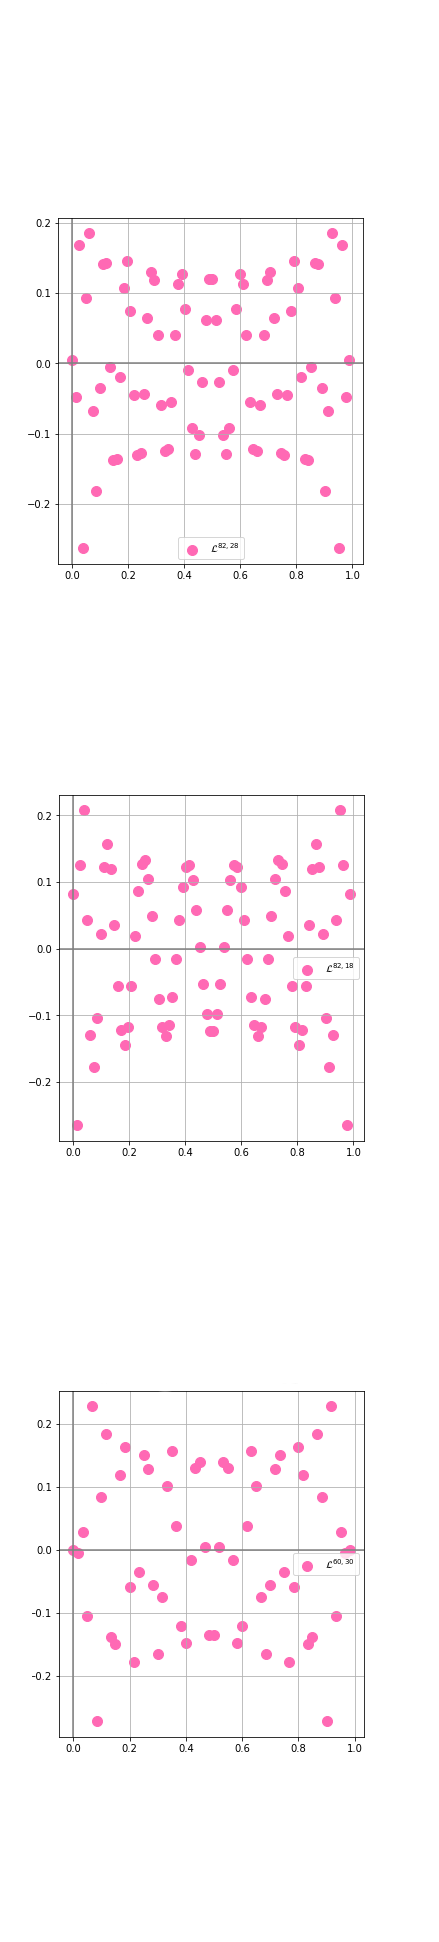
\includegraphics[scale=1.3]{portada_tesis2} 
\end{marginfigure}






\vspace{4cm}

\noindent
\textsc{Tesis} \\
que para obtener el grado de \\
\textsc{licenciada en matemáticas} \\
presenta \\
\textsc{Denisse Amélie Sophie Bernès Carmona}



\vspace{2cm}

\noindent
Asesor: \textsc{Dr. Moisés Soto Bajo} \\
Co-asesor: \textsc{Dr. Javier Herrera Vega} 




\vspace*{\fill}
Puebla, Pue. Junio del 2023 







%Texto usado para la imagen lateral. 
%\textsc{Dimensión $n$}\\
%\vspace{1cm}
%\underline{\textsc{Señales constantes, $W_{n,0}$.}}\\
%\vspace{1cm}
%\underline{\textsc{Señales afines, $W_{n,1}$.}}\\
%\vspace{1cm}
%\underline{\textsc{Señales cuadráticas, $W_{n,2}$.}}\\
%\vspace{1cm}
%\underline{\textsc{Señales $n$-dimensionales, $W_{n,n-1}$.}} \\
%\vspace{1cm}
%$\vdots$

%\vspace{5cm}

\newpage